\section{Наибольшее и наименьшее значение функции нескольких переменных в области}
Решите задачу, составив и исследовав функцию нескольких переменных на наибольшее / наименьшее значение в области. Поиск условного экстремума не требуется.



\subsection{Постановка задачи}
В прямой эллиптический конус, полуоси основания которого A и B,
высота H, вписана призма с прямоугольным основанием так, что
стороны основания параллельны осям, а пересечение диагоналей
основания лежит в центре эллипса. Каковы должны быть стороны
основания и высота этой призмы, чтобы её объём был наибольшим?
Каков этот наибольший объём?
\begin{figure}[H]
\centering
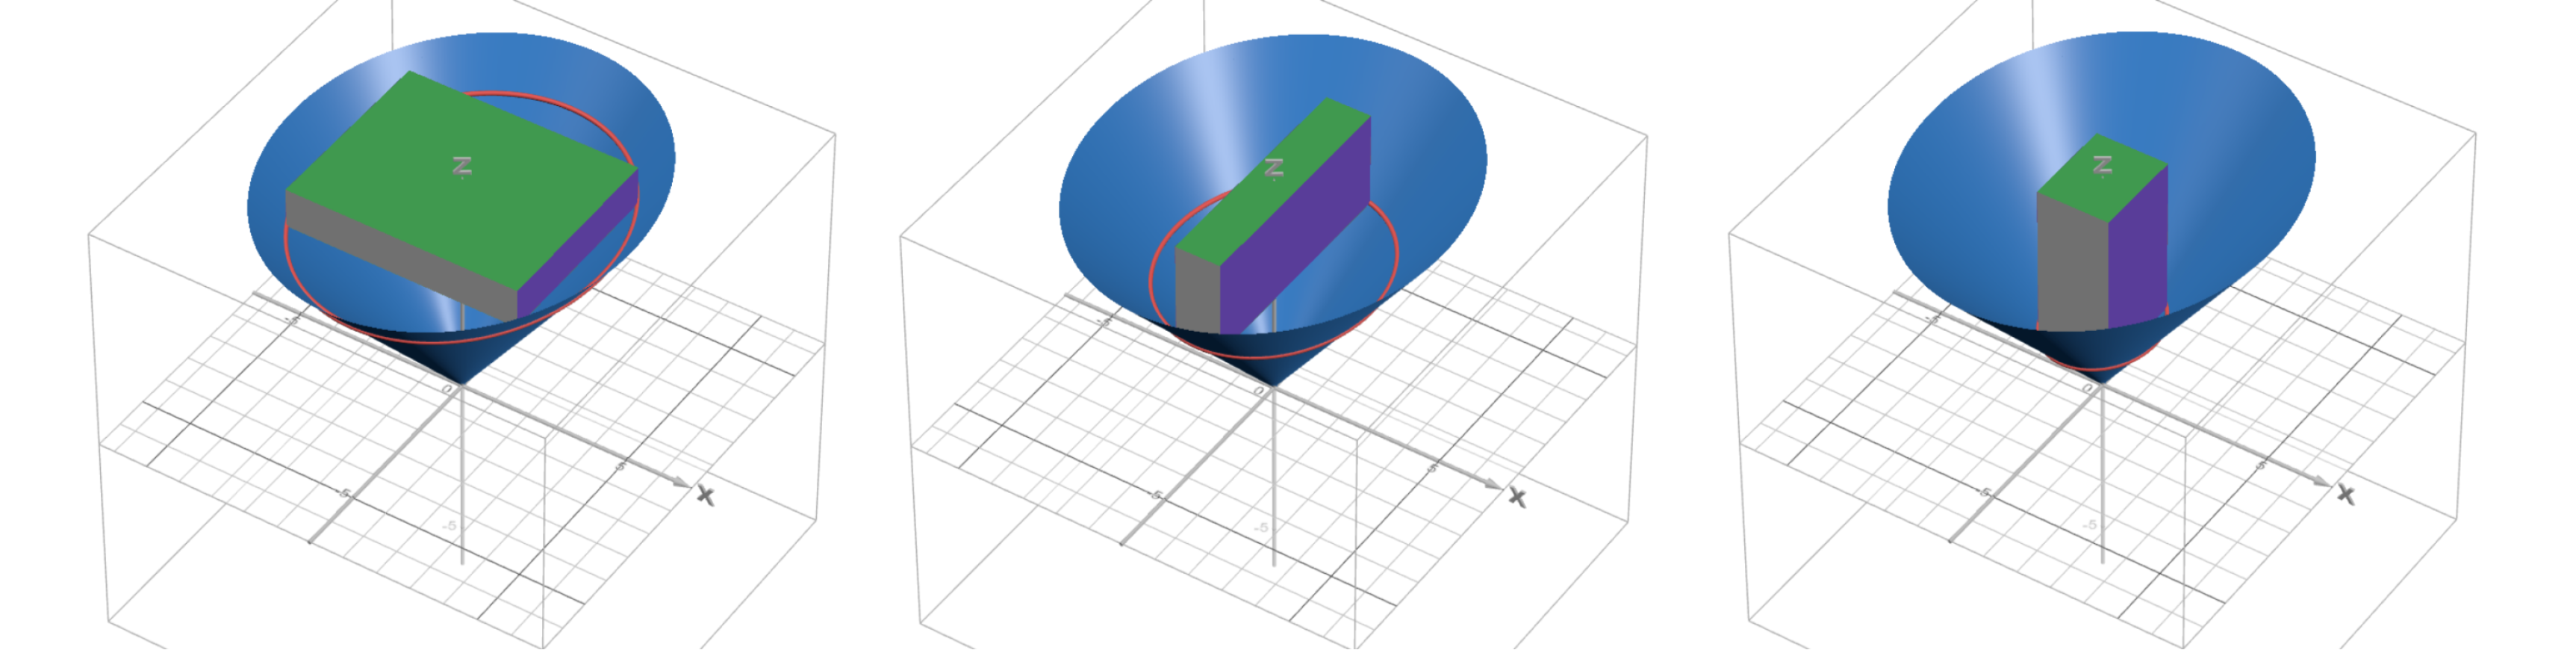
\includegraphics[width=1\textwidth]{img/ex.png}
\caption{Примеры призмы, вписанной в конус}
\end{figure}





\subsection{Объём призмы, вписанной в конус}
Объем призмы вычисляется по формуле
$$V = S_{\text{осн}} \cdot h,$$
где $S_{\text{осн}}$ - площадь основания, $h$ - высота призмы.\\
Расположим вершину конуса в начале координат. Тогда уравнение конической поверхности примет канонический вид:
$$
\frac{x^2}{a^2} + \frac{y^2}{b^2} = \frac{z^2}{c^2}
$$

Нас интересует не вся коническая поверхность, а только ее верхняя часть, ограниченная плоскостью $z = H$.
$$
\frac{x^2}{A^2} + \frac{y^2}{B^2} = \frac{z^2}{H^2}, \; 0 \leq z \leq H
$$
Призма вписана в конус. Это значит, что одно её основание лежит в плоскости $z = H$. Другое - на некоторой высоте, в плоскости $z = z_0$, и вершины этого основания лежат на образующих конуса. $z_0$ - это варьируемый параметр, ненулевое расстояние от начала координат до нижнего основания. Тогда высота полученнной призмы есть $(H - z_0)$.\\

Рассмторим сечение конуса плоскостью $z = z_0, \; 0 < z_0 < H$. В сечении ожидаемо получится эллипс:
$$
\frac{x^2}{A^2 \cdot \frac{z_0^2}{H^2}} + \frac{y^2}{B^2 \cdot \frac{z_0^2}{H^2}} = 1
$$
Введем обозначения полуосей эллипса, полученного в результате такого сечения:
$$
a(z_0) =  \frac{A}{H} z_0, \; b(z_0) =  \frac{B}{H} z_0,
$$
Уравнение эллипса приняло более компактный вид:
$$
\frac{x^2}{a(z_0)^2} + \frac{y^2}{b(z_0)^2} = 1
$$
Точки нижнего основания призмы лежат на этом эллипсе. Известно, что основание призмы представляет собой прямоугольник, пересечение диагоналей которого лежит в центре эллипса. Если одна из вершин задается точкой $(x_0, y_0)$, то оставшиеся три вершины задаются точками: $(-x_0, y_0)$, $(-x_0, -y_0)$, $(x_0, -y_0)$.
\begin{figure}[H]
\centering
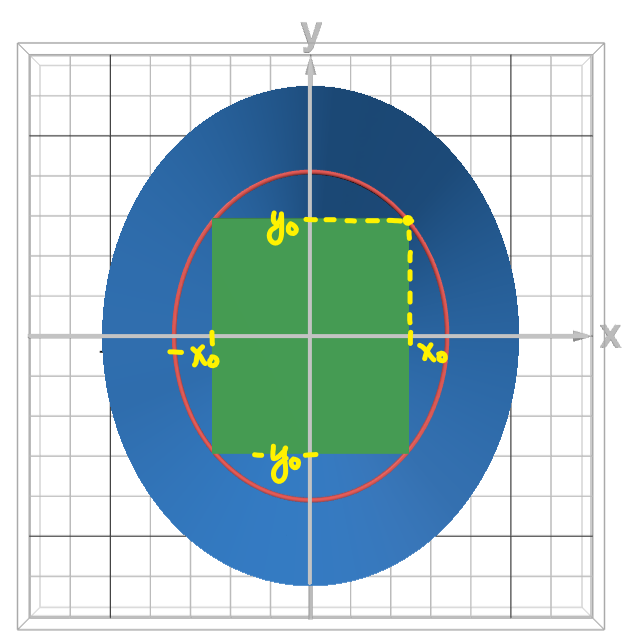
\includegraphics[width=0.6\textwidth]{img/up.png}
\caption{Вид сверху}
\end{figure}
В силу симметри примем значения $x_0$ и $y_0$ строго положительными. Тогда длины сторон такого прямоугольника равны $2x_0$ и $2y_0$, а площадь $S_{\text{осн}} = 4x_0y_0$.

Вспомним, что вершины прямоугольника принадлежат эллипсу. Тогда при фиксации варьируемого параметра $x_0, 0 < x_0 < a(z_0)$ получим единственное значение $y_0$. Найдем его:
$$
\frac{x_0^2}{a(z_0)^2} + \frac{y_0^2}{b(z_0)^2} = 1
$$
$$
y_0^2 = b(z_0)^2 \frac{a(z_0)^2 - x_0^2}{a(z_0)^2}
$$
$$
y_0 = \frac{B}{A} \sqrt{\frac{A^2}{H^2} z_0^2 - x_0^2} 
$$

Таким образом, запишем выражение для объема призмы, вписанной в конус.
$$
V = S_{\text{осн}} \cdot h = 4x_0y_0(H-z_0)
$$
$$
V(z_0, x_0) = 4x_0\frac{B}{A} \sqrt{\frac{A^2}{H^2} z_0^2 - x_0^2} (H - z_0)
$$
Или, если ввести обозначение для корня:
$$
V(z_0, x_0) = 4\frac{B}{A} x_0 K (H - z_0), \; K = \sqrt{\frac{A^2}{H^2} z_0^2 - x_0^2}
$$
Область определения: 
$$
0 < z_0 < H, \; 0 < x_0 < \frac{A}{H}z_0
$$




\subsection{Поиск максимума функции}
Максимум функции достигается в точке максимума. По необходимуму условию экстремума точки экстремума нужно искать среди критических точек функции. Для нахождения критических точек возьмем частные производные функции объёма призмы:
$$
\frac{\partial V}{\partial z_0} = 4\frac{B}{A} x_0 
\left( 
\frac{2\frac{A^2}{H^2}z_0}{2K} (H-z_0) - K
\right) 
$$

$$
\frac{\partial V}{\partial x_0} = 4\frac{B}{A} (H-z_0) 
\left( 
K - x_0 \frac{2x_0}{2K}
\right) 
$$
Эти производные существуют и не обращаются в бексонечность на всей области определения:
$$
0 < z_0 < H, \; 0 < x_0 < \frac{A}{H}z_0
$$
Поэтому задача по нахождению критических точек сводится к нахождению стационарных точек. Найдем такие точки, в которых обе производные равны нулю одновременно. Начнем рассмотрение с частной производной по $x_0$.
$$
4\frac{B}{A} (H-z_0) 
\left( 
K - x_0 \frac{2x_0}{2K}
\right) = 0
$$
$$
(H-z_0) 
\left( 
K^2 - x_0^2
\right) = 0
$$
$$
(H-z_0) 
\left( 
\frac{A^2}{H^2} z_0^2 - x_0^2 - x_0^2
\right) = 0
$$
$$
z_0 = H - \text{не входит в ОДЗ}
$$
$$
x_0 = - \frac{1}{\sqrt{2}}\frac{A}{H}z_0 - \text{не входит в ОДЗ}
$$
$$
x_0 = \frac{1}{\sqrt{2}}\frac{A}{H}z_0
$$
Подставим найденное значение $x_0$ в частную производную по $z_0$:
$$
4\frac{B}{A} x_0 
\left( 
\frac{2\frac{A^2}{H^2}z_0}{2K} (H-z_0) - K
\right) = 0
$$
$$
x_0 
\left( 
\frac{A^2}{H^2}z_0 (H-z_0) - K^2
\right) = 0
$$
$$
x_0 
\left( 
\frac{A^2}{H^2}z_0 (H-z_0) - \frac{A^2}{H^2} z_0^2 + x_0^2
\right) = 0
$$
$$
\frac{1}{\sqrt{2}}\frac{A}{H}z_0 
\left( 
\frac{A^2}{H^2}z_0 (H-z_0) - \frac{A^2}{H^2} z_0^2 + \frac{1}{2}\frac{A^2}{H^2}z_0^2
\right) = 0
$$
$$
z_0^2
\left( 
H-z_0 - z_0 + \frac{1}{2}z_0
\right) = 0
$$
$$
z_0^2
\left( 
H - \frac{3}{2}z_0
\right) = 0
$$
$$
z_0 = 0 - \text{не входит в ОДЗ}
$$
$$
z_0 = \frac{2}{3}H
$$
$$
x_0 = \frac{1}{\sqrt{2}}\frac{A}{H} z_0 = \frac{\sqrt{2}}{3}A
$$
Нашли единственную стационарную точку для нашей ОДЗ. Проверим, что она является точкой максимума.\\
Воспользуемся достаточным условием экстремума функции двух переменных для стационораной точки. Для начала вычилим значения вторых частных производных функции $V$ в точке исследуемой точке $M(z_0 = \frac{2}{3}H; \; x_0 = \frac{\sqrt{2}}{3}A)$.
$$
\frac{\partial V}{\partial z_0} = 4\frac{B}{A} x_0 
\left( 
\frac{A^2}{H^2}z_0 (H-z_0) - K^2
\right) \frac{1}{K}
$$

$$
\frac{\partial V}{\partial x_0} = 4\frac{B}{A} (H-z_0) 
\left( 
K^2 - x_0^2
\right) \frac{1}{K}
$$
$$
K_M = \sqrt{\frac{A^2}{H^2} \frac{4}{9}H^2 - \frac{2}{9}A^2} = \frac{\sqrt{2}A}{3} = x_{0_M}
$$
$$
(H-z_0)_M = H - \frac{2}{3}H = \frac{1}{3}H
$$
Так как ислледуемая точка $M$ является стационарной,
$$
\left( 
\frac{A^2}{H^2}z_0 (H-z_0) - K^2
\right)_M = 0 \text{ и }
\left( 
K^2 - x_0^2
\right)_M = 0
$$
то вид вторых частных производных $V$ в точке $M$ упрощается, останутся только те слагаемые, где взяты производные от этих "скобочек".
$$
\frac{\partial^2 V}{\partial z_0^2} (M) = 4\frac{B}{A} x_0 
\left( 
\frac{A^2}{H^2}z_0H - \frac{A^2}{H^2}z_0^2 - \frac{A^2}{H^2} z_0^2 + x_0^2
\right)'_{z_0} \frac{1}{K} = 
$$
$$
= 4\frac{BA}{H^2} x_0 
\left( 
-4z_0 + H
\right)\frac{1}{K} =  
4\frac{BA}{H^2} 
\left( 
-\frac{8H}{3} + H
\right) = 
$$
$$
= -\frac{20}{3}\frac{AB}{H} = \cal A
$$


$$
\frac{\partial^2 V}{\partial x_0^2} = 4\frac{B}{A} (H-z_0) 
\left( 
\frac{A^2}{H^2}z_0^2 - 2x_0^2
\right)'_{x_0} \frac{1}{K} = 
$$
$$
= 4\frac{B}{A} \frac{H}{3} 
\left( 
 - 4x_0
\right) \frac{1}{K} = -\frac{16}{3}\frac{BH}{A} = \cal C
$$


$$
\frac{\partial^2 V}{\partial x_0 \partial z_0} = 4\frac{B}{A} (H-z_0) 
\left( 
\frac{A^2}{H^2}z_0^2 - 2x_0^2
\right)'_{z_0} \frac{1}{K} = 
$$
$$
= 4\frac{B}{A} (H-z_0) 
\left( 
2\frac{A^2}{H^2}z_0
\right) \frac{1}{K} = 
4\frac{B}{A} \frac{H}{3}
2\frac{A^2}{H^2} \frac{2H}{3}
 \frac{3}{\sqrt{2}A} =
$$
$$
= \frac{16}{3\sqrt{2}}B = \cal B
$$
$$
\cal D = \cal A \cal C - \cal B ^{\text{2}} = 
$$
$$
= -\frac{20}{3}\frac{AB}{H} \cdot -\frac{16}{3}\frac{BH}{A} - \frac{16 \cdot 16}{18}B^2 = \frac{20 \cdot 16 \cdot 2}{18}B^2 - \frac{16 \cdot 16}{18}B^2
$$
Так как $\cal D$ $> 0$ и $\cal A$ $< 0$, то по достаточному условию экстремума функции двух переменных для стационораной точки точка $M(z_0 = \frac{2}{3}H; \; x_0 = \frac{\sqrt{2}}{3}A)$ является точкой максимума.

\subsection{Конечный результат}
Высота полученной призмы:
$$
h = H - z_0 = \frac{H}{3}
$$
Стороны основания:
$$
a = 2x_0 = \frac{2\sqrt{2}}{3}A
$$
$$
b = 2y_0 = \frac{B}{A} K_M = 2 \frac{B}{A} \frac{\sqrt{2}}{3}A = \frac{2 \sqrt{2}}{3}B
$$
Максимальный объем призмы, вписанной в конус:
$$
V = a \cdot b \cdot h = \frac{8}{27}ABH
$$

\begin{figure}[H]
\centering
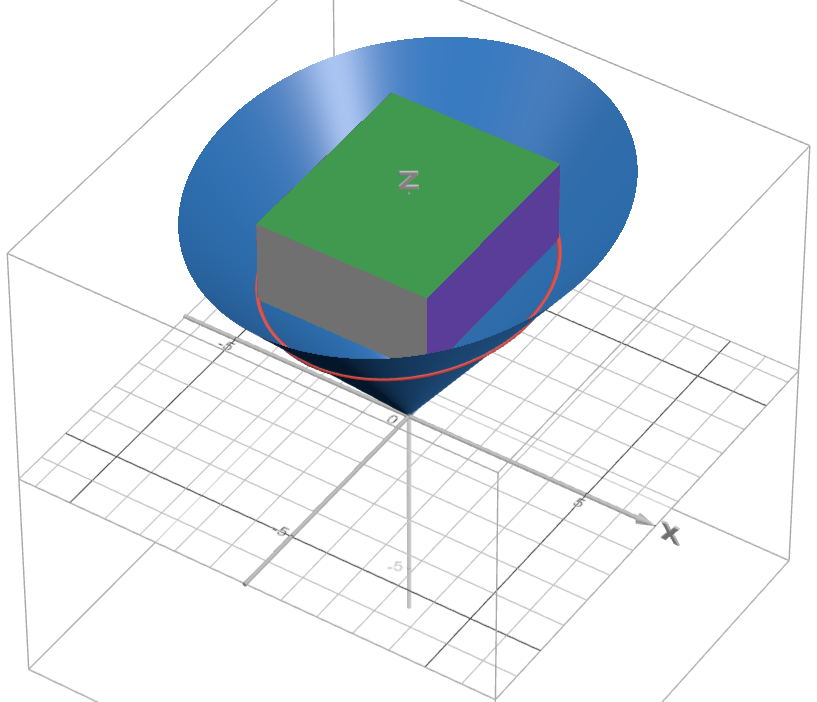
\includegraphics[width=0.6\textwidth]{img/res.png}
\caption{Итоговый результат. \href{https://www.desmos.com/3d/88d50f8402}{[интерактивный пример в редакторе Desmos 3D]}}
\end{figure}
